\chapter{SYSTEM DESIGN}

\section{Overview}
The system design represents the structural and functional aspects of the proposed system, illustrating how different components interact. This section covers various Unified Modeling Language (UML) diagrams, which define the system's architecture and workflow.

\section{Use Case Diagram}
The use case diagram provides an overview of system interactions, depicting different user roles and their associated functionalities.

\begin{figure}[H]
    \centering
    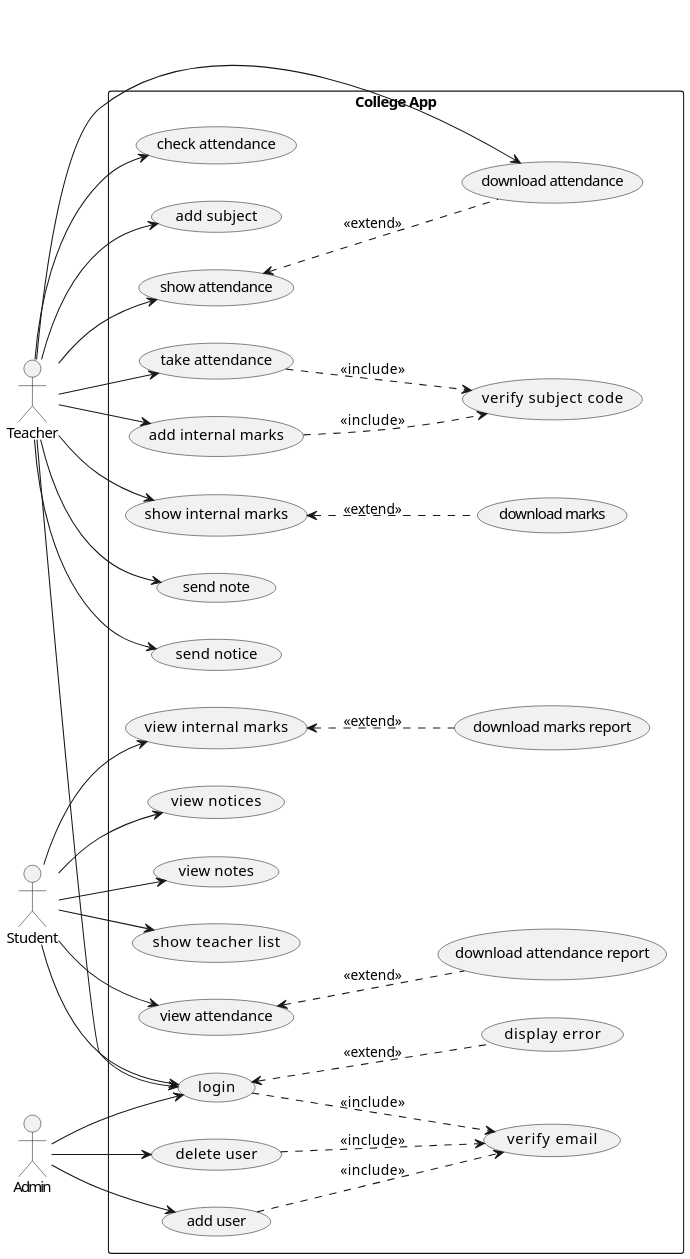
\includegraphics[width=0.8\textwidth]{Graphics/usecase_diagarm.png}
    \caption{Use Case Diagram}
    \label{fig:use_case_diagram}
\end{figure}

\section{Class Diagram}
The class diagram represents the object-oriented structure of the system, defining various classes, attributes, methods, and relationships between them.

\begin{figure}[H]
    \centering
    \includegraphics[width=1\textwidth]{Graphics/class_diagram.png}
    \caption{Class Diagram}
    \label{fig:class_diagram}
\end{figure}

\section{Sequence Diagrams}
Sequence diagrams illustrate the interaction between objects over time for different scenarios. Below are three key scenarios:

\subsection{Scenario 1: User Authentication}
\begin{figure}[H]
    \centering
    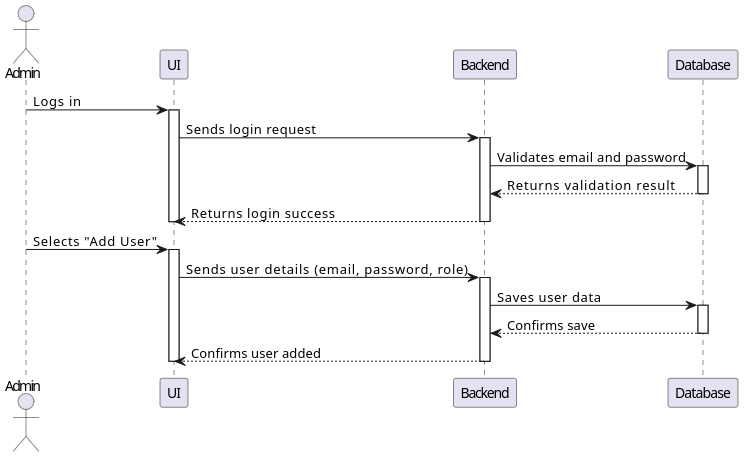
\includegraphics[width=0.8\textwidth]{Graphics/sequence_Diagram_Case_1Admin_adds_User.drawio.png}
    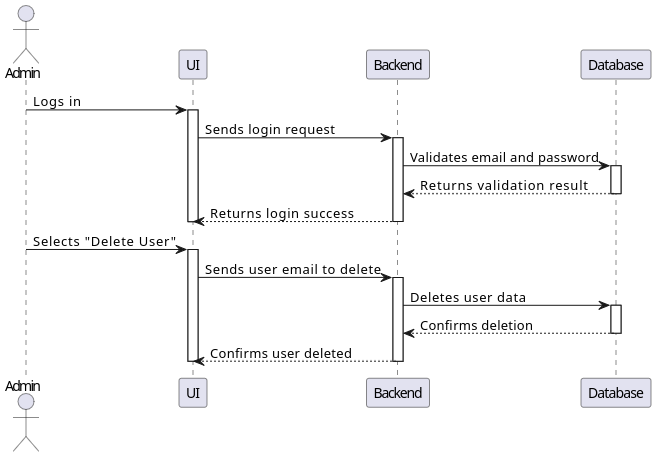
\includegraphics[width=0.8\textwidth]{Graphics/sequence_diagram_Admin_Deletes_User.drawio.png}
    \caption{Sequence Diagram for User Authentication}
    \label{fig:sequence_diagram_authentication}
\end{figure}

\subsection{Scenario 2: Attendance Management}
\begin{figure}[H]
    \centering
    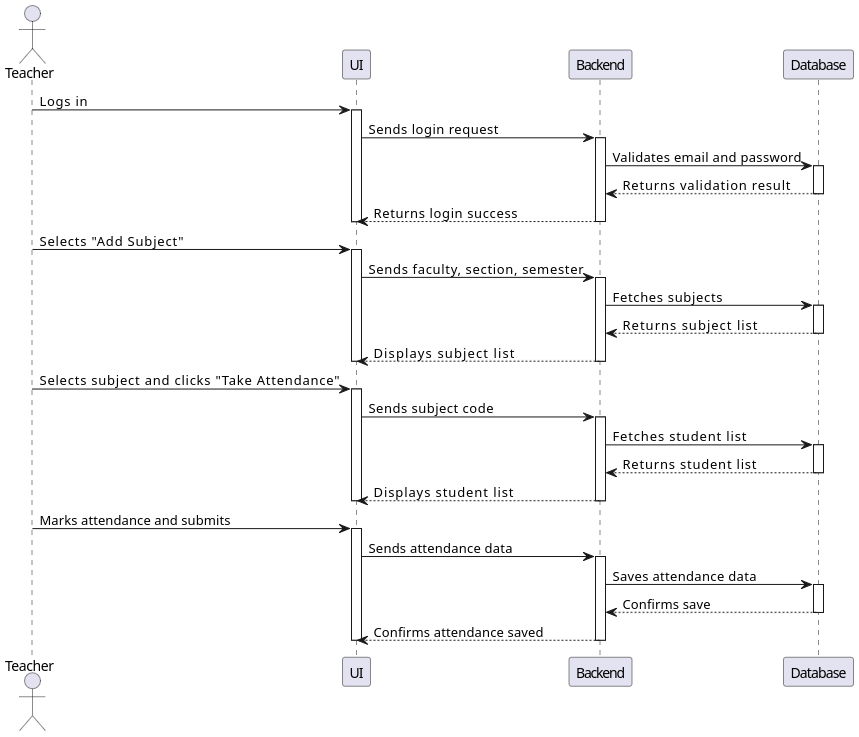
\includegraphics[width=0.8\textwidth]{Graphics/Sequence_Diagram_Teacher_Takes_Attendance.png}
    \caption{Sequence Diagram for Attendance Management}
    \label{fig:sequence_diagram_attendance}
\end{figure}

\subsection{Scenario 3: Viewing Marks and Notices}
\begin{figure}[H]
    \centering
    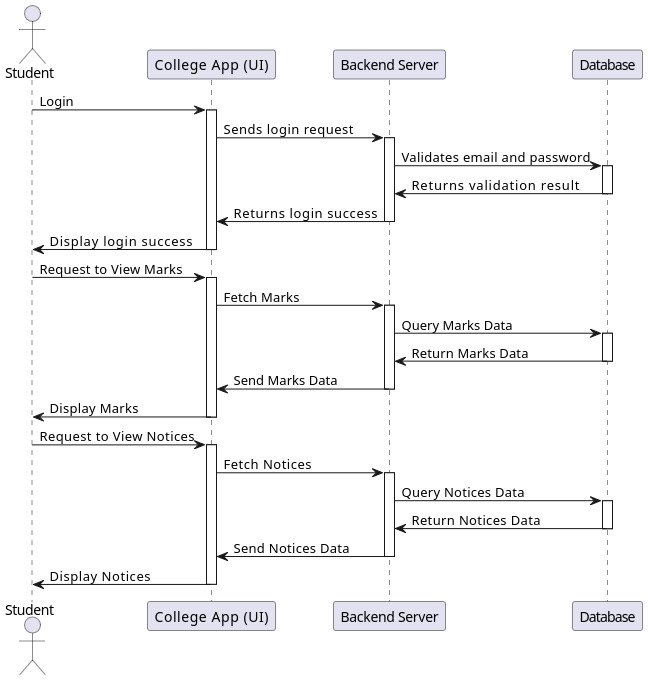
\includegraphics[width=0.8\textwidth]{Graphics/seq_dig_for_viewing_marks_and_attendance.jpg}
    \caption{Sequence Diagram for Viewing Marks and Notices}
    \label{fig:sequence_diagram_marks_notices}
\end{figure}

\section{Activity Diagrams}
Activity diagrams model the workflows for different functionalities, showing the sequence of operations. Below are three key workflows:

\subsection{Scenario 1: User Login Process}
\begin{figure}[H]
    \centering
    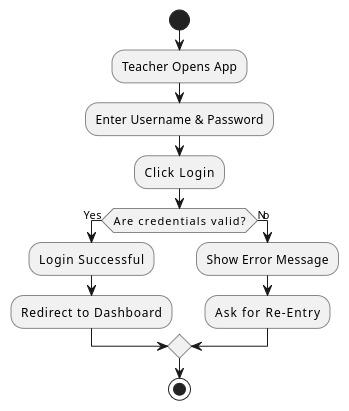
\includegraphics[width=0.8\textwidth]{Graphics/activity_diagram_teacher_login.jpg}
    \caption{Activity Diagram for Login Process}
    \label{fig:activity_diagram_login}
\end{figure}

\subsection{Scenario 2: Data Entry by Teachers}
\begin{figure}[H]
    \centering
    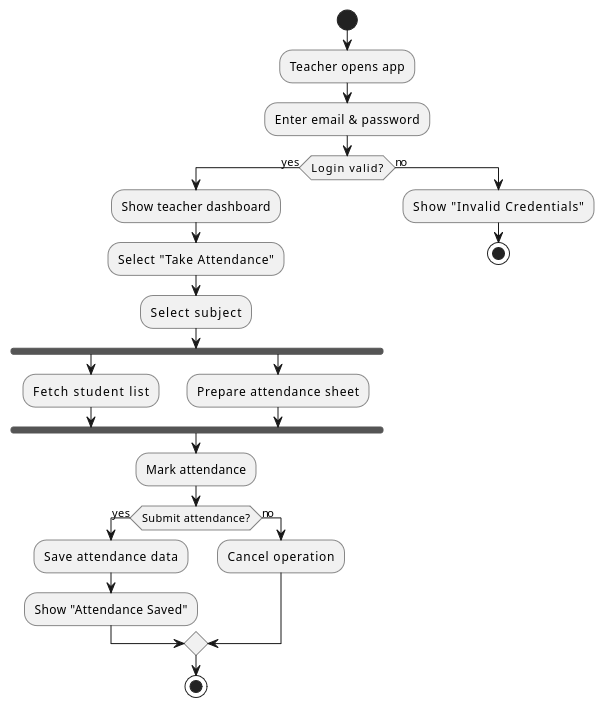
\includegraphics[width=0.8\textwidth]{Graphics/Activity_Diagram_teacher_takes_attendance.png}
    \caption{Activity Diagram for Attendance Entry}
    \label{fig:activity_diagram_data_entry}
\end{figure}

\subsection{Scenario 3: Students Viewing Results}
\begin{figure}[H]
    \centering
    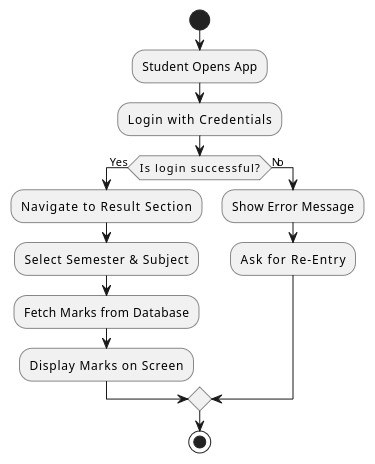
\includegraphics[width=0.8\textwidth]{Graphics/viewresult.jpg}
    \caption{Activity Diagram for Viewing Results}
    \label{fig:activity_diagram_viewing_results}
\end{figure}

\section{Component Diagram}
The component diagram outlines the system's physical structure, illustrating dependencies between different components such as the front-end, back-end, database, and external APIs.

\begin{figure}[H]
    \centering
    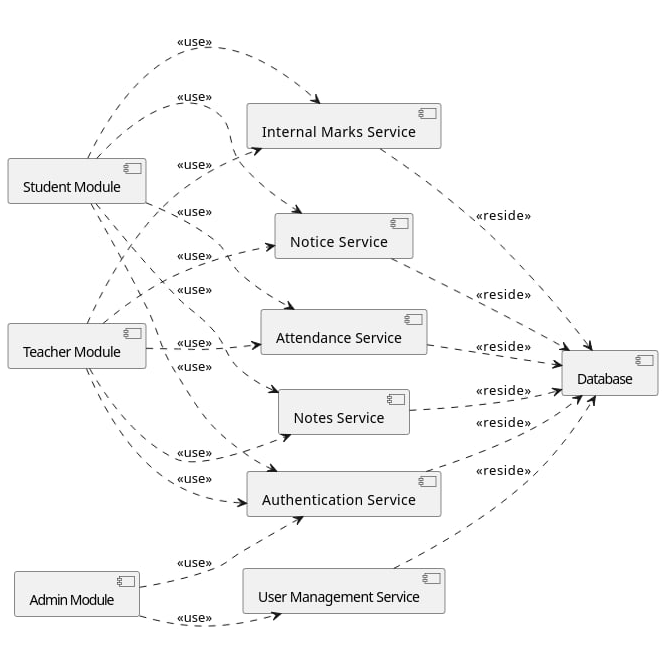
\includegraphics[width=0.8\textwidth]{Graphics/component_diagram.png}
    \caption{Component Diagram}
    \label{fig:component_diagram}
\end{figure}